\documentclass[a4paper,12pt]{article}

\usepackage{float}


\usepackage[utf8]{inputenc}
\usepackage[dvips]{graphicx}
%\usepackage{a4wide}
\usepackage{epsfig}
\usepackage{fancybox}
\usepackage{verbatim}
\usepackage{array}
\usepackage{latexsym}
\usepackage{alltt}
\usepackage{amssymb}
\usepackage{amsmath,amsthm}
\usepackage{bm}
\usepackage{wasysym}

%\usepackage{fullpage}
%\usepackage{hyperref}
\usepackage{listings}
\usepackage{color}
\usepackage{algorithm}
\usepackage{algpseudocode}
\usepackage[hmargin=2cm,vmargin=3.0cm]{geometry}
%\topmargin=0cm
%\topmargin=-1.8cm
%\addtolength{\textheight}{6.5cm}
%\addtolength{\textwidth}{2.0cm}
%\setlength{\leftmargin}{-3cm}
%\setlength{\oddsidemargin}{0.0cm}
%\setlength{\evensidemargin}{0.0cm}

%misc libraries goes here
\usepackage{tikz}
\usepackage{tikz-qtree}
\usetikzlibrary{automata,positioning}

\usepackage{multicol}
\usepackage{enumitem}

\usepackage[most]{tcolorbox}

\usepackage[colorlinks=true,urlcolor=black,linkcolor=black]{hyperref}


\lstdefinestyle{customtex}{
    %backgroundcolor=\color{lbcolor},
    tabsize=2,
    language=TeX,
    numbers=none,
    basicstyle=\footnotesize\ttfamily,
    numberstyle=\footnotesize,
    aboveskip={0.0\baselineskip},
    belowskip={0.0\baselineskip},
    %
    columns=flexible,
    keepspaces=true,
    fontadjust=true,
    upquote=true,
    %
    breaklines=true,
    prebreak=\raisebox{0ex}[0ex][0ex]{\ensuremath{\hookleftarrow}},
    frame=single,
    showtabs=false,
    showspaces=false,
    showstringspaces=false,
    %
    %identifierstyle=\color[rgb]{0,0.2,0.8},
    identifierstyle=\color[rgb]{0,0,0.5},
    %identifierstyle=\color[rgb]{0.133,0.545,0.133},
    %keywordstyle=\color[rgb]{0.8,0,0},
    %keywordstyle=\color[rgb]{0.133,0.545,0.133},
    keywordstyle=\color[rgb]{0,0,0.5},
    %commentstyle=\color[rgb]{0.133,0.545,0.133},
    commentstyle=\color[rgb]{0.545,0.545,0.545},
    %stringstyle=\color[rgb]{0.827,0.627,0.133},
    stringstyle=\color[rgb]{0.133,0.545,0.133},
    %
    literate={â}{{\^{a}}}1 {Â}{{\^{A}}}1 {ç}{{\c{c}}}1 {Ç}{{\c{C}}}1 {ğ}{{\u{g}}}1 {Ğ}{{\u{G}}}1 {ı}{{\i}}1 {İ}{{\.{I}}}1   {ö}{{\"o}}1 {Ö}{{\"O}}1 {ş}{{\c{s}}}1 {Ş}{{\c{S}}}1 {ü}{{\"u}}1 {Ü}{{\"U}}1 {~}{$\sim$}{1}
}

\lstdefinestyle{output}{
    %backgroundcolor=\color{lbcolor},
    tabsize=2,
    numbers=none,
    basicstyle=\footnotesize\ttfamily,
    numberstyle=\footnotesize,
    aboveskip={0.0\baselineskip},
    belowskip={0.0\baselineskip},
    %
    columns=flexible,
    keepspaces=true,
    fontadjust=true,
    upquote=true,
    %
    breaklines=true,
    prebreak=\raisebox{0ex}[0ex][0ex]{\ensuremath{\hookleftarrow}},
    frame=single,
    showtabs=false,
    showspaces=false,
    showstringspaces=false,
    %
    %identifierstyle=\color[rgb]{0.44,0.12,0.1},
    identifierstyle=\color[rgb]{0,0,0},
    keywordstyle=\color[rgb]{0,0,0},
    commentstyle=\color[rgb]{0,0,0},
    stringstyle=\color[rgb]{0,0,0},
    %
    literate={â}{{\^{a}}}1 {Â}{{\^{A}}}1 {ç}{{\c{c}}}1 {Ç}{{\c{C}}}1 {ğ}{{\u{g}}}1 {Ğ}{{\u{G}}}1 {ı}{{\i}}1 {İ}{{\.{I}}}1   {ö}{{\"o}}1 {Ö}{{\"O}}1 {ş}{{\c{s}}}1 {Ş}{{\c{S}}}1 {ü}{{\"u}}1 {Ü}{{\"U}}1
}

\lstset{style=customtex}


\tikzset{%
    terminal/.style={draw, rectangle,
    				 align=center, 
					 minimum height=1cm, 
					 minimum width=2cm,
					 fill=black!10,
					 anchor=mid},
    nonterminal/.style={draw, rectangle,
    					align=left,
					    minimum height=1cm, 
						minimum width=2cm, 
						anchor=mid},% and so on
}

%% Style for terminals
%\tikzstyle{terminal}=[draw, rectangle, 
%					  minimum height=1cm, 
%					  minimum width=2cm, 
%					  fill=black!20,
%					  anchor=south west]
%% Style for nonterminals
%\tikzstyle{nonterminal}=[draw, rectangle, 
%						 minimum height=1 cm, 
%						 minimum width=2 cm, 
%						 anchor=north east]


\newcommand{\HRule}{\rule{\linewidth}{1mm}}
\newcommand{\kutu}[2]{\framebox[#1mm]{\rule[-2mm]{0mm}{#2mm}}}
\newcommand{\gap}{ \\[1mm] }

\newcommand{\Q}{\raisebox{1.7pt}{$\scriptstyle\bigcirc$}}
\newcommand{\minus}{\scalebox{0.35}[1.0]{$-$}}

\setlength{\fboxsep}{10pt}

\tcbsetforeverylayer{enhanced jigsaw, breakable, arc=0mm, boxrule=1pt, boxsep=5pt, after=\vspace{1em}, colback=white, colframe=black}

\newcolumntype{P}[1]{>{\centering\arraybackslash}p{#1}}

\setlength\parindent{0pt}

%\renewcommand\arraystretch{1.2}

\newenvironment{Tab}[1]
  {\def\arraystretch{1}\tabular{#1}}
  {\endtabular}

%%%%%%%%%%%%%%%%%%%%%%%%%%%%%%%%%%%%%%%%%%%%%%%%%%%%%%%%%%%%%%%%%%%%%%%%%%%%%%%%%%%%%%

\title{Formal Languages and Abstract Machines \\ Take Home Exam 2}
\author{Yavuz Selim YESILYURT \\ 2259166} % write your name and id
\date{} % do not write any date

%%%%%%%%%%%%%%%%%%%%%%%%%%%%%%%%%%%%%%%%%%%%%%%%%%%%%%%%%%%%%%%%%%%%%%%%%%%%%%%%%%%%%%

\begin{document}
\HRule\\
Middle East Technical University \hfill Department of Computer Engineering
{\let\newpage\relax\maketitle}
\HRule\\
\vspace{1cm}

%%%%%%%%%%%%%%%%%%%%%%%%%%%%%%%%%%%%%%%%%%%%%%%%%%%%%%%%%%%%%%%%%%%%%%%%%%%%%%%%%%%%%%

% Write your answers below the section tags
\section{Context-Free Grammars \hfill \normalfont{(10 pts)}}

\paragraph{a)} Give the rules of the Context-Free Grammars to recognize strings in the given languages where $\Sigma=\{a,b\}$ and $S$ is the start symbol. \\  

$L(G)=\{w \mid \;  w \in \Sigma^*;\; |w| \geq 3;\; $  \hfill \small{(2/10 pts)} \\
\hspace*{22mm} the first and the second from the last symbols of $w$ are the same$\}$ \\

\begin{tcolorbox}
S $\rightarrow$ aXaA $|$ bXbA \\
X $\rightarrow$ aX $|$ bX $|$ e \\
A $\rightarrow$ a $|$ b \\
\end{tcolorbox}


$L(G)=\{w \mid \;  w \in \Sigma^*;\; $ the length of w is odd$\}$ \hfill \small{(2/10 pts)} \\

\begin{tcolorbox}
S $\rightarrow$ aX $|$ bX \\
X $\rightarrow$ aS $|$ bS $|$ e \\
\end{tcolorbox}


$L(G)=\{w \mid \;  w \in \Sigma^*;\; n(w,a)=2\cdot n(w,b)\}$ where $n(w,x)$ is the number of $x$ symbols in $w$ \hfill \small{(3/10 pts)} \\

\begin{tcolorbox}
S $\rightarrow$ aaSbS $|$ bSaaS $|$ abSaS $|$  baSaS $|$ aSabS $|$ aSbaS $|$ e\\
\end{tcolorbox}



\paragraph{b)} Find the set of strings recognized by the CFG rules given below:         \hfill \small{(3/10 pts)} \\


$S \to X \mid Y$ \\
$X \to aXb \mid A \mid B$ \\
$A \to aA \mid a$ \\
$B \to Bb \mid b$ \\
$Y \to CbaC$ \\
$C \to CC \mid a \mid b \mid \varepsilon$  \\

\begin{tcolorbox}
$L(G)=\{w \mid \;  w \in \{a,b\}^*;\; contains \ ba \ or \ in \ the \ form \ a^xb^y \ where \ x \neq y,\ x,y\geq 1 \}$
\end{tcolorbox}


\newpage
\section{Parse Trees and Derivations \hfill \normalfont{(20 pts)}}
Given the CFG below, provide parse trees for given sentences in \textbf{a} and \textbf{b}.\\

\begin{lstlisting}[style=output,mathescape=true]
S   $\to$ NP VP
VP  $\to$ V NP | V NP PP
PP  $\to$ P NP
NP  $\to$ N | D N | NP PP
V   $\to$ wrote | built | constructed
D   $\to$ a | an | the | my
N   $\to$ John | Mary | Jane | man | book | automata | pen | class
P   $\to$ in | on | by | with
\end{lstlisting}

\paragraph{a)} Jane constructed automata with a pen \hfill \small{(4/20 pts)} \\

\begin{tcolorbox}
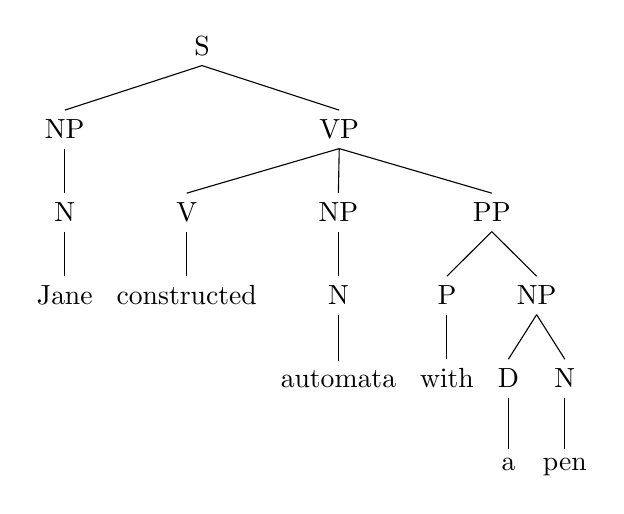
\begin{tikzpicture}[scale=1]
\Tree [.S [.NP [.N Jane ] ] [.VP [.V constructed ] [.NP [.N automata ] ] [.PP [.P with ] [.NP [.D a ] [.N pen ] ] ] ] ]
\end{tikzpicture}
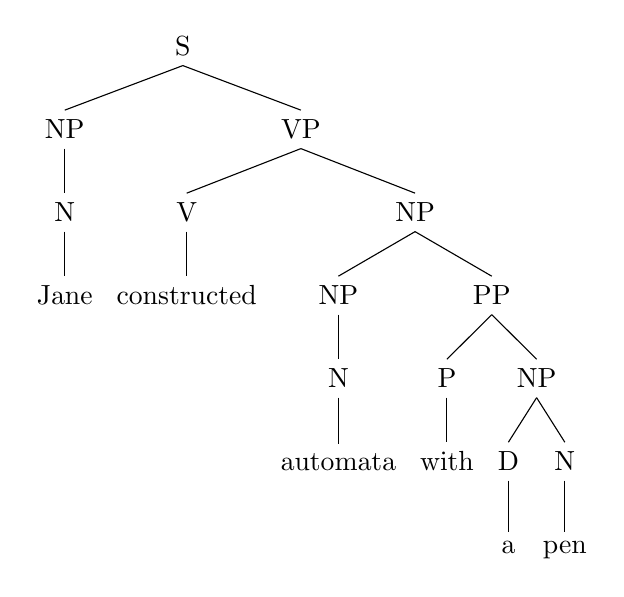
\begin{tikzpicture}[scale=1]
\Tree [.S [.NP [.N Jane ] ] [.VP [.V constructed ] [.NP [.NP [.N automata ] ] [.PP [.P with ] [.NP [.D a ] [.N pen ] ] ] ] ] ]
\end{tikzpicture}
\end{tcolorbox}
\newpage
\paragraph{b)} my book in the man built a Jane by a pen \hfill \small{(4/20 pts)} \\
\begin{tcolorbox}
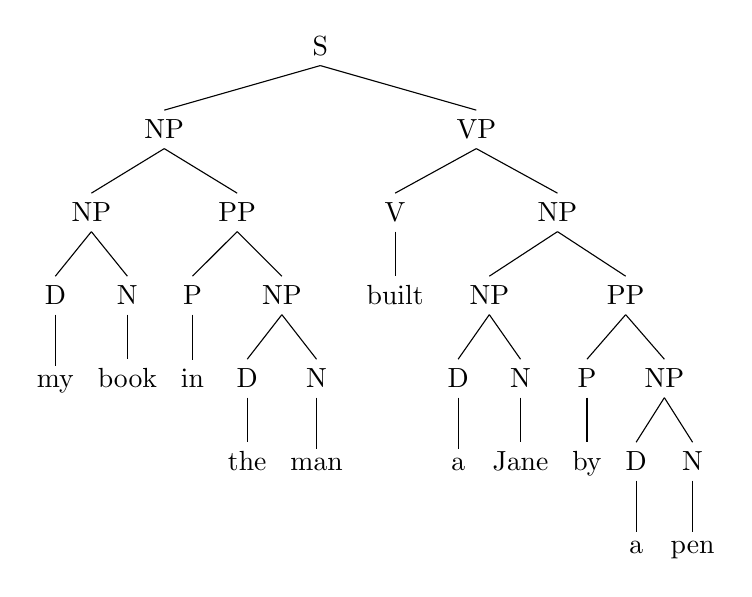
\begin{tikzpicture}[scale=1]
\Tree [.S [.NP [.NP [.D my ] [.N book ] ] [.PP [.P in ] [.NP [.D the ] [.N man ] ] ] ] [.VP [.V built ] [.NP [.NP [.D a ] [.N Jane ] ] [.PP [.P by ] [.NP [.D a ] [.N pen ] ] ] ] ] ]
\end{tikzpicture}

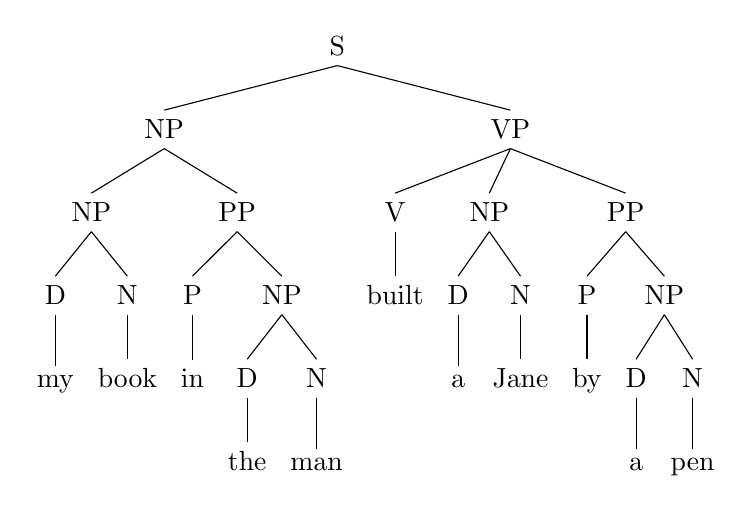
\begin{tikzpicture}[scale=1]
\Tree [.S [.NP [.NP [.D my ] [.N book ] ] [.PP [.P in ] [.NP [.D the ] [.N man ] ] ] ] [.VP [.V built ] [.NP [.D a ] [.N Jane ] ] [.PP [.P by ] [.NP [.D a ] [.N pen ] ] ] ] ]
\end{tikzpicture}
\end{tcolorbox}
\newpage

Given the CFG below, answer \textbf{c}, \textbf{d} and \textbf{e} \\

\begin{lstlisting}[style=output,mathescape=true]
S  $\to$ E
E  $\to$ E + T | E - T | T
T  $\to$ T * I | T / I | I
I  $\to$ 0 | 1 | 2 | 3 | 4 | 6 | 7 | 8 | 9
\end{lstlisting}

\paragraph{c)} Provide the left-most derivation of 7 - 4 * 3 step-by-step and plot the final parse \hfill \small{(4/20 pts)} \\
tree matching that derivation \\
\begin{tcolorbox}
Left-most derivation:\\
S $\Rightarrow$ E $\Rightarrow$ E - T $\Rightarrow$ T - T $\Rightarrow$ I - T $\Rightarrow$ 7 - T $\Rightarrow$ 7 - T * I $\Rightarrow$ 7 - I * I $\Rightarrow$ 7 - 4 * I $\Rightarrow$ 7 - 4 * 3 \\\\
Corresponding parse tree:\\
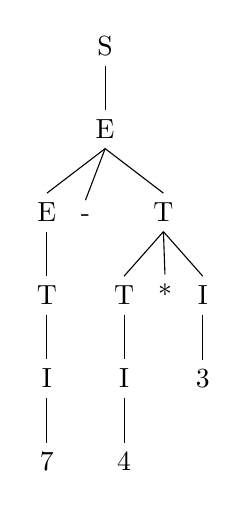
\begin{tikzpicture}[scale=1]
\Tree [.S [.E [.E [.T [.I $7$ ] ] ] [.- ] [.T [.T [.I $4$ ] ] [.* ] [.I $3$ ] ] ] ]
\end{tikzpicture}
\end{tcolorbox}

\paragraph{d)} Provide the right-most derivation of 7 - 4 * 3 step-by-step and plot the final parse \hfill \small{(4/20 pts)} \\
 tree matching that derivation \\
\newpage
\begin{tcolorbox}
Right-most derivation:\\
S $\Rightarrow$ E $\Rightarrow$ E - T $\Rightarrow$ E - T * I $\Rightarrow$ E - T * 3 $\Rightarrow$ E - I * 3 $\Rightarrow$ E - 4 * 3 $\Rightarrow$ T - 4 * 3 $\Rightarrow$ I - 4 * 3 $\Rightarrow$ 7 - 4 * 3\\\\
Corresponding parse tree:\\
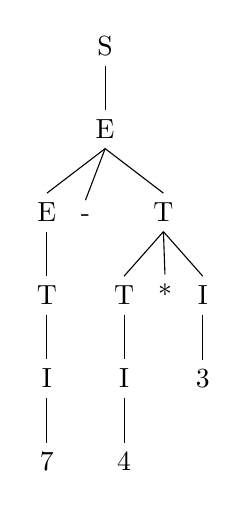
\begin{tikzpicture}[scale=1]
\Tree [.S [.E [.E [.T [.I $7$ ] ] ] [.- ] [.T [.T [.I $4$ ] ] [.* ] [.I $3$ ] ] ] ]
\end{tikzpicture}
\end{tcolorbox}


\paragraph{e)} Are the derivations in \textbf{c} and \textbf{d} in the same similarity class?  \hfill \small{(4/20 pts)} \\
\begin{tcolorbox}
Yes, because from the definition, we say, two derivations $D$ and $D'$ are similar if the pair $(D,D')$ belongs in the reflexive, symmetric, transitive closure of $\prec$. In other words two derivations are similar if they can be transformed into another via a sequence of "switchings" in the order in which rules are applied. Such a "switching" can replace a derivation either by one that precedes it, or by one that it precedes. In our example we found a left-most derivation and a right-most derivation for a word with the rules given. As can be seen clearly, we can reach to the right-most derivation via a sequence of "switchings" on left-most derivation and vice-versa applies. Besides two derivations gave us the same parse trees, which implies that these derivations are in the same similarity class.
\end{tcolorbox}



\newpage
\section{Pushdown Automata \hfill \normalfont{(30 pts)}}

\paragraph{a)} 
Find the language recognized by the PDA given below \hfill \small{(5/30 pts)} \\

\begin{tikzpicture}[shorten >=1pt,node distance=3cm,on grid,auto]
\node[state,initial,initial text=] (q_0) {$q_0$};
\node[state] (q_1) [right=of q_0] {$q_1$};
\node[state] (q_2) [above right=of q_1] {$q_2$};
\node[state] (q_3) [below right=of q_1] {$q_3$};
\node[state,accepting](q_4) [right=of q_2] {$q_4$};
\node[state](q_5) [right=of q_3] {$q_5$};
\node[state,accepting](q_6) [right=of q_5] {$q_6$};
\path[->]

(q_0) edge node {$\varepsilon,\varepsilon \to \#$} (q_1)
(q_1) edge [loop below] node {$x,\varepsilon \to x$} (q_1)

%%
(q_1) edge node {$\varepsilon,\varepsilon \to \varepsilon$} (q_2)
(q_2) edge [loop above] node {$y,x \to \varepsilon$} (q_2)

(q_2) edge node {$\varepsilon,\# \to \varepsilon$} (q_4)
(q_4) edge [loop above] node {$z,\varepsilon \to \varepsilon$} (q_4)

%%%

(q_1) edge node {$\varepsilon,\varepsilon \to \varepsilon$} (q_3)
(q_3) edge [loop below] node {$y,\varepsilon \to \varepsilon$} (q_3)

(q_3) edge node {$\varepsilon,\varepsilon \to \varepsilon$} (q_5)
(q_5) edge [loop below] node {$z,x \to \varepsilon$} (q_5)

(q_5) edge node {$\varepsilon,\# \to \varepsilon$} (q_6)
;
\end{tikzpicture} \\

\begin{minipage}{0.60\textwidth}
where the transition $((q_i,\alpha,\beta),(q_j,\gamma)) $ is represented as: 
\end{minipage}
\begin{minipage}{0.30\textwidth}
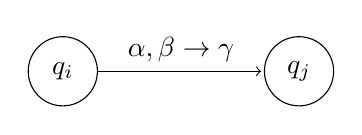
\begin{tikzpicture}[shorten >=1pt,node distance=3cm,on grid,auto]
\node[state] (q_i) {$q_i$};
\node[state] (q_j) [right=of q_i] {$q_j$};
\path[->]
(q_i) edge node {$\alpha,\beta \to \gamma$} (q_j);
\end{tikzpicture} \\
\end{minipage}


\begin{tcolorbox}
Language recognized by the PDA above is:\\
$ L=\{x^n y^n z^m \ or \ x^n y^m z^n  \mid \; n,m \geq 0; \; n,m \in \mathbb{N}  \} $ 
\end{tcolorbox}


\paragraph{b)} 
Design a PDA to recognize language $ L=\{x^n y^{m+n} x^m \mid \; n,m \geq 0; \; n,m \in \mathbb{N}  \} $  \hfill \small{(5/30 pts)} \\
\begin{tcolorbox}
\begin{center}
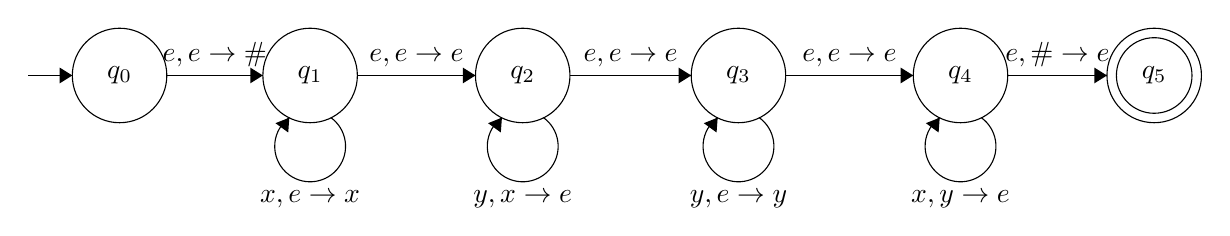
\begin{tikzpicture}[scale=0.2]
\tikzstyle{every node}+=[inner sep=0pt]
\draw [black] (6.9,-25) circle (3);
\draw (6.9,-25) node {$q_0$};
\draw [black] (19,-25) circle (3);
\draw (19,-25) node {$q_1$};
\draw [black] (32.5,-25) circle (3);
\draw (32.5,-25) node {$q_2$};
\draw [black] (46.2,-25) circle (3);
\draw (46.2,-25) node {$q_3$};
\draw [black] (60.3,-25) circle (3);
\draw (60.3,-25) node {$q_4$};
\draw [black] (72.6,-25) circle (3);
\draw (72.6,-25) node {$q_5$};
\draw [black] (72.6,-25) circle (2.4);
\draw [black] (1.1,-25) -- (3.9,-25);
\fill [black] (3.9,-25) -- (3.1,-24.5) -- (3.1,-25.5);
\draw [black] (9.9,-25) -- (16,-25);
\fill [black] (16,-25) -- (15.2,-24.5) -- (15.2,-25.5);
\draw (12.95,-24.5) node [above] {$e,e\rightarrow \# $};
\draw [black] (20.323,-27.68) arc (54:-234:2.25);
\draw (19,-32.25) node [below] {$x,e\rightarrow x$};
\fill [black] (17.68,-27.68) -- (16.8,-28.03) -- (17.61,-28.62);
\draw [black] (22,-25) -- (29.5,-25);
\fill [black] (29.5,-25) -- (28.7,-24.5) -- (28.7,-25.5);
\draw (25.75,-24.5) node [above] {$e,e\rightarrow e$};
\draw [black] (33.823,-27.68) arc (54:-234:2.25);
\draw (32.5,-32.25) node [below] {$y,x\rightarrow e$};
\fill [black] (31.18,-27.68) -- (30.3,-28.03) -- (31.11,-28.62);
\draw [black] (35.5,-25) -- (43.2,-25);
\fill [black] (43.2,-25) -- (42.4,-24.5) -- (42.4,-25.5);
\draw (39.35,-24.5) node [above] {$e,e\rightarrow e$};
\draw [black] (47.523,-27.68) arc (54:-234:2.25);
\draw (46.2,-32.25) node [below] {$y,e\rightarrow y$};
\fill [black] (44.88,-27.68) -- (44,-28.03) -- (44.81,-28.62);
\draw [black] (49.2,-25) -- (57.3,-25);
\fill [black] (57.3,-25) -- (56.5,-24.5) -- (56.5,-25.5);
\draw (53.25,-24.5) node [above] {$e,e\rightarrow e$};
\draw [black] (61.623,-27.68) arc (54:-234:2.25);
\draw (60.3,-32.25) node [below] {$x,y\rightarrow e$};
\fill [black] (58.98,-27.68) -- (58.1,-28.03) -- (58.91,-28.62);
\draw [black] (63.3,-25) -- (69.6,-25);
\fill [black] (69.6,-25) -- (68.8,-24.5) -- (68.8,-25.5);
\draw (66.45,-24.5) node [above] {$e, \# \rightarrow e$};
\end{tikzpicture}
\end{center}
\end{tcolorbox}
\newpage

\paragraph{c)} 
Design a PDA to recognize language $ L=\{x^n y^m \mid \; n < m \leq 2n; \; n,m \in \mathbb{N^+} \} $  \hfill \small{(10/30 pts)} \\
Do not use multi-symbol push/pop operations in your transitions. \\
Simulate the PDA on strings \textit{xxy} (with only one rejecting derivation) and \textit{xxyyyy} (accepting derivation) with transition tables. \\
\begin{tcolorbox}
Let $M = (K,\Sigma ,\Gamma ,\Delta ,s,F)$, where $K = \{q_0,q_1,q_2,q_3,q_4\}$, $\Sigma=\{x,y\}$, $\Gamma = \{x,y\}$, $s = q_0$, $F = \{q_4\}$ and $\Delta$ contains eight transitions;\\
\begin{center}
1.$((q_0,e,e),(q_1,\# ))$\\
2.$((q_1,x,e),(q_1,x))$\\
3.$((q_1,y,e),(q_2,e))$\\
4.$((q_2,y,x),(q_2,e))$\\
5.$((q_2,y,x),(q_3,e))$\\
6.$((q_2,e,\# ),(q_4,e))$\\
7.$((q_3,y,e),(q_2,e))$\\
8.$((q_3,e,\# ),(q_4,e))$\\
\end{center}
The PDA figure is given below;\\
\begin{center}
\begin{tikzpicture}[scale=0.2]
\tikzstyle{every node}+=[inner sep=0pt]
\draw [black] (6.9,-25) circle (3);
\draw (6.9,-25) node {$q_0$};
\draw [black] (27.8,-25) circle (3);
\draw (27.8,-25) node {$q_1$};
\draw [black] (47.3,-25) circle (3);
\draw (47.3,-25) node {$q_2$};
\draw [black] (27.8,-48.2) circle (3);
\draw (27.8,-48.2) node {$q_3$};
\draw [black] (72.6,-25) circle (3);
\draw (72.6,-25) node {$q_4$};
\draw [black] (72.6,-25) circle (2.4);
\draw [black] (1.1,-25) -- (3.9,-25);
\fill [black] (3.9,-25) -- (3.1,-24.5) -- (3.1,-25.5);
\draw [black] (9.9,-25) -- (24.8,-25);
\fill [black] (24.8,-25) -- (24,-24.5) -- (24,-25.5);
\draw (17.35,-24.5) node [above] {$e,e\rightarrow \# $};
\draw [black] (26.477,-22.32) arc (234:-54:2.25);
\draw (27.8,-17.75) node [above] {$x,e\rightarrow x$};
\fill [black] (29.12,-22.32) -- (30,-21.97) -- (29.19,-21.38);
\draw [black] (30.8,-25) -- (44.3,-25);
\fill [black] (44.3,-25) -- (43.5,-24.5) -- (43.5,-25.5);
\draw (37.55,-24.5) node [above] {$y,e\rightarrow e$};
\draw [black] (45.977,-22.32) arc (234:-54:2.25);
\draw (47.3,-17.75) node [above] {$y,x\rightarrow e$};
\fill [black] (48.62,-22.32) -- (49.5,-21.97) -- (48.69,-21.38);
\draw [black] (28.249,-45.235) arc (168.16863:111.73611:26.639);
\fill [black] (28.25,-45.24) -- (28.9,-44.55) -- (27.92,-44.35);
\draw (33.38,-32.12) node [left] {$y,x\rightarrow e$};
\draw [black] (50.3,-25) -- (69.6,-25);
\fill [black] (69.6,-25) -- (68.8,-24.5) -- (68.8,-25.5);
\draw (59.95,-24.5) node [above] {$e,\# \rightarrow e$};
\draw [black] (71.507,-27.793) arc (-23.71654:-101.52805:36.575);
\fill [black] (71.51,-27.79) -- (70.73,-28.32) -- (71.64,-28.73);
\draw (61.71,-46.08) node [below] {$e,\# \rightarrow e$};
\draw [black] (47.582,-27.984) arc (1.07306:-81.16832:19.845);
\fill [black] (47.58,-27.98) -- (47.1,-28.79) -- (48.1,-28.77);
\draw (43.48,-42.56) node [right] {$y,e\rightarrow e$};
\end{tikzpicture}
\end{center}

For the \textit{xxy} simulation;\\
	\begin{table}[H]
	\small
	\centering
	\begin{tabular}{|c|c|c|c|}	
	\hline
	$State$ & $Unread \ Input$ & $Stack$ & $Transition \ Used$\\
	\hline 
	$q_0$ & $xxy$ & $e$ & -\\			
	$q_1$ & $xxy$ & $\# $ & 1\\	
	$q_1$ & $xy$  & $x\# $ & 2\\
	$q_1$ & $y$   & $xx\# $ & 2\\
	$q_2$ & $e$   & $xx\# $ & 3\\	
	\hline 
	\end{tabular}
	\end{table}
As can be seen in the last row of the transition table, input word ended but stack is not empty and the machine is not in the final state, since there is not a suitable transition for that case in our PDA the word is not accepted by the Language.\\

For the \textit{xxyyyy} simulation;\\
	\begin{table}[H]
	\small
	\centering
	\begin{tabular}{|c|c|c|c|}	
	\hline
	$State$ & $Unread \ Input$ & $Stack$ & $Transition \ Used$\\
	\hline 
	$q_0$ & $xxyyyy$ & $e$ & -\\			
	$q_1$ & $xxyyyy$ & $\# $ & 1\\	
	$q_1$ & $xyyyy$  & $x\# $ & 2\\
	$q_1$ & $yyyy$   & $xx\# $ & 2\\
	$q_2$ & $yyy$   & $xx\# $ & 3\\	
	$q_3$ & $yy$ & $x\# $ & 5\\			
	$q_2$ & $y$ & $x\# $ & 7\\	
	$q_3$ & $e$  & $\# $ & 5\\
	$q_4$ & $e$   & $e$ & 8\\
	\hline 
	\end{tabular}
	\end{table}
As can be seen in the last row of the transition table, input word and stack contents are empty and the machine is in final state, therefore word is accepted by the language.
\end{tcolorbox}

\paragraph{d)} Given two languages $L'$ and $L$ as $L'=\{w \mid \; w\in L; \; |w|=4n+2 \; for\; n\in \mathbb{N} \}$
\hfill \small{(10/30 pts)} \\
If $L$ is a CFL, show that $L'$ is also a CFL by constructing an automaton for $L'$ in terms of another automaton that recognizes $L$. \\
\newpage
\begin{tcolorbox}
If $L$ is a CFL then it has a push down automata that recognizes $L$ with its alphabets, transitions and states. To construct an automaton for $L'$ in terms of another automaton that recognizes $L$ we will make some additions on the CFL of $L$ and get the final automata. So lets say $L$ has a PDA $M = (K,\Sigma ,\Gamma ,\Delta ,s,F)$, where $K$ contains some states including its initial state and final state(s), let $s = q_0$ and $\Delta$ contains some transitions.\\\\
To construct the automata that recognizes both languages we will design a PDA for $L'$ and then bind it with the PDA of $L$ with adding a new state and adding transitions to it for both languages, namely we will create a new initial state for final automata and add two transitions to it to combine these PDA'S. So let us illustrate that;\\

\begin{center}
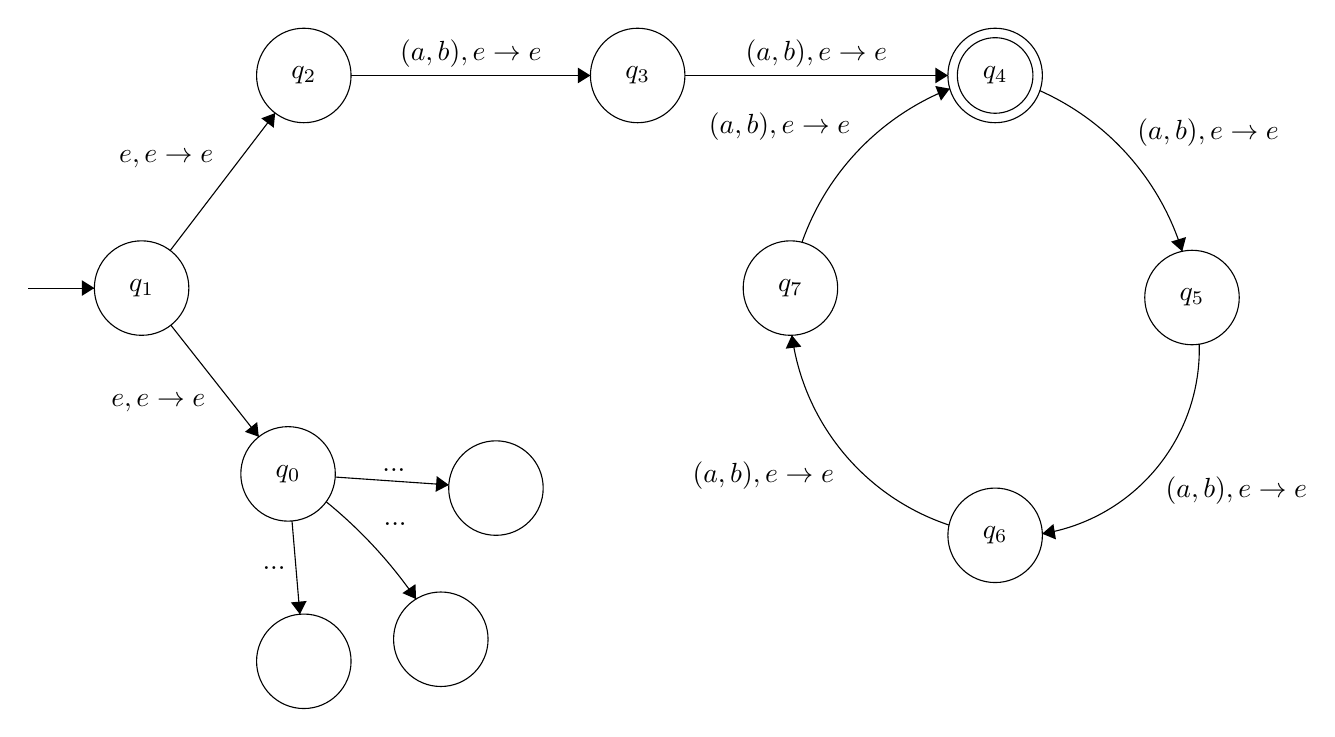
\begin{tikzpicture}[scale=0.2]
\tikzstyle{every node}+=[inner sep=0pt]
\draw [black] (8.2,-27.9) circle (3);
\draw (8.2,-27.9) node {$q_1$};
\draw [black] (17.5,-39.7) circle (3);
\draw (17.5,-39.7) node {$q_0$};
\draw [black] (18.5,-14.4) circle (3);
\draw (18.5,-14.4) node {$q_2$};
\draw [black] (39.7,-14.4) circle (3);
\draw (39.7,-14.4) node {$q_3$};
\draw [black] (62.4,-14.4) circle (3);
\draw (62.4,-14.4) node {$q_4$};
\draw [black] (62.4,-14.4) circle (2.4);
\draw [black] (74.9,-28.5) circle (3);
\draw (74.9,-28.5) node {$q_5$};
\draw [black] (62.4,-43.6) circle (3);
\draw (62.4,-43.6) node {$q_6$};
\draw [black] (49.4,-27.9) circle (3);
\draw (49.4,-27.9) node {$q_7$};
\draw [black] (27.2,-50.2) circle (3);
\draw [black] (30.7,-40.6) circle (3);
\draw [black] (18.5,-51.6) circle (3);
\draw [black] (10.02,-25.51) -- (16.68,-16.79);
\fill [black] (16.68,-16.79) -- (15.8,-17.12) -- (16.59,-17.72);
\draw (12.78,-19.75) node [left] {$e,e\rightarrow e$};
\draw [black] (10.06,-30.26) -- (15.64,-37.34);
\fill [black] (15.64,-37.34) -- (15.54,-36.41) -- (14.76,-37.03);
\draw (12.28,-35.22) node [left] {$e,e\rightarrow e$};
\draw [black] (1,-27.9) -- (5.2,-27.9);
\fill [black] (5.2,-27.9) -- (4.4,-27.4) -- (4.4,-28.4);
\draw [black] (21.5,-14.4) -- (36.7,-14.4);
\fill [black] (36.7,-14.4) -- (35.9,-13.9) -- (35.9,-14.9);
\draw (29.1,-13.9) node [above] {$(a,b),e\rightarrow e$};
\draw [black] (42.7,-14.4) -- (59.4,-14.4);
\fill [black] (59.4,-14.4) -- (58.6,-13.9) -- (58.6,-14.9);
\draw (51.05,-13.9) node [above] {$(a,b),e\rightarrow e$};
\draw [black] (65.236,-15.365) arc (65.99112:17.12445:16.483);
\fill [black] (74.28,-25.57) -- (74.52,-24.66) -- (73.57,-24.95);
\draw (71.4,-18.03) node [right] {$(a,b),e\rightarrow e$};
\draw [black] (75.359,-31.457) arc (1.57602:-80.81293:11.868);
\fill [black] (65.39,-43.5) -- (66.26,-43.86) -- (66.1,-42.88);
\draw (73.19,-40.79) node [right] {$(a,b),e\rightarrow e$};
\draw [black] (59.477,-42.95) arc (-108.35671:-172.39204:14.762);
\fill [black] (49.49,-30.89) -- (49.1,-31.75) -- (50.09,-31.62);
\draw (52.2,-39.79) node [left] {$(a,b),e\rightarrow e$};
\draw [black] (50.133,-24.995) arc (160.58105:111.5808:16.326);
\fill [black] (59.52,-15.24) -- (58.6,-15.07) -- (58.96,-16);
\draw (53.24,-17.63) node [left] {$(a,b),e\rightarrow e$};
\draw [black] (20.49,-39.9) -- (27.71,-40.4);
\fill [black] (27.71,-40.4) -- (26.94,-39.84) -- (26.87,-40.84);
\draw (24.22,-39.57) node [above] {$...$};
\draw [black] (19.921,-41.47) arc (50.91892:34.54517:29.527);
\fill [black] (25.63,-47.65) -- (25.59,-46.7) -- (24.76,-47.27);
\draw (23.53,-42.89) node [right] {$...$};
\draw [black] (17.75,-42.69) -- (18.25,-48.61);
\fill [black] (18.25,-48.61) -- (18.68,-47.77) -- (17.68,-47.86);
\draw (17.38,-45.71) node [left] {$...$};
\end{tikzpicture}
\end{center}

$q_1$ is the initial state of the automata that recognizes both languages and as can be seen from the figure above it has two $e$ transitions to $q_2$ and $q_0$ representing automata that recognizes $L'$ and automata that recognizes $L$ respectively. Since we do not know the contents of the language $L$, I just added an $e$ transition from the initial state $q_1$ to its older initial state $q_0$ and I left the other transitions and states related with $L$ blank, which means they can be in any form that will construct the PDA for recognizing $L$.
\end{tcolorbox}

\newpage
\section{Closure Properties \hfill \normalfont{(20 pts)}}

Let $L_1$ and $L_2$ be context-free languages which are not regular, and let $L_3$ be a regular language. Determine whether the following languages are necessarily CFLs or not. If they need to be context-free, explain your reasoning. If not, give one example where the language is a CFL and a counter example where the language is not a CFL. \\

\paragraph{a)} $L_4 = L_1 \cap (L_2 \setminus L_3)$ \hfill \small{(10/20 pts)} \\

\begin{tcolorbox}
$L_2-L_3$ also equals to $L_2\cap L_3'$, since $L_3$ is a regular language, its closed under complementation so $L_3'$ is also a regular language. We also know that the intersection of a Context-free language and a regular language is Context-free, therefore we can say $L_2 \cap L_3'$ (also $L_2-L_3$) is context-free. We know the intersection of two CFL is not necessarily Context-free, so since $L_1$ and the righthand-side are Context free we can not say $L_4$ is necessarily context-free. For example in the case of $L_1=\{a^nb^nc^m | m,n \geq 0\}$ and rhs equals to $\{a^nb^mc^m | m,n \geq 0\}$, $L_4 = \{a^nb^nc^n | n \geq 0\}$ which is not a Context-free language, but for example in the case of $L_1=\{a^nb^n | n \geq 0\}$ and rhs equals to $\{a^{2n}b^{2n} | n \geq 0\}$, $L_4 = \{a^nb^n | n \geq 0\}$ which is a Context-free language.
\end{tcolorbox}

\paragraph{b)} $L_5 = (L_1 \cap L_3)\text{*}$ \hfill \small{(10/20 pts)} \\

\begin{tcolorbox}
$L_1$ is a CFL and $L_3$ is a Regular Language, since we know that the intersection of a CFL and a regular language is context-free, we can easily say that intersection of $L_1$ and $L_3$ is context-free and since the CFL are closed under Kleene Star operation, the Kleene star of the expression is also context-free, therefore $L_5$ is context-free.
\end{tcolorbox}





\newpage
\section{Pumping Theorem \hfill \normalfont{(20 pts)}}

\paragraph{a)} Show that $L=\{a^n m^n t^i \mid \; n\leq i \leq 2n\}$ is not a Context Free Language \hfill \small{(10/20 pts)} \\
using Pumping Theorem for CFLs. \\

\begin{tcolorbox}
Assume that $L$ is a CFL, Then by Pumping Lemma there exists a pumping length $k$, depending on the grammar, such that any word $w \in L$ of length greater than $k$ can be re-written as $w=uvxyz$ for $v \neq e$ or $y \neq e$. We will apply the strong version of the lemma which additionally says $|vxy|<k$ . Let our $w=a^km^kt^{2k}$ and we have $|vy|\geq 1$ and $|vxy| < k$. Depending on the where we pump $vxy$ to $w$ there are 5 cases.\\\\
Cases 1 and 2: We can either pump $vxy$ for $i=1$ within the $a$'s on the first part of the word ($vxy$ only consists of $a$'s) or within the $m$'s on the second part of the word ($vxy$ only consists of $m$'s) , and in each case we get: $w'=a^xm^yt^{2k}$ (in case 1 $x=k+1 ,\ y=k$, in case 2 $x=k ,\ y=k+1$) where $x\neq y$, which constitutes a contradiction.\\\\
For case 3: We can pump $vxy$ to the third part of the word which consists of only $t$'s. In this case, when we pump $vxy$ with $i=1$, we get $w'=a^km^kt^x$, where $x > 2k$ namely $x = 2k + 1$ which contradicts with the form of the word.\\\\
For case 4: We can pump $vxy$ in between first and second part of the word, namely it can contain some $a$'s and some $m$'s. In this case if we pump $vxy$ for $i=0$ we get, $w'=a^xm^yt^{2k}$ where either $x\neq y$ or if they are equal $2x < 2k$ which creates a contradiction.\\\\
For case 5: We can pump $vxy$ in between second and third part of the word, namely it can contain some $m$'s and some $t$'s. In this case if we pump $vxy$ for $i=0$ we get, $w'=a^km^xt^y$ where either $k\neq x$ or if they are equal $y < 2k$ which creates a contradiction.\\\\

In each case we reached to a contradiction, therefore we can say $L$ is not Context Free Language.
\end{tcolorbox}

\newpage

\paragraph{b)} Show that $L=\{a^n b^{2n} a^n \mid \; n \in \mathbb{N+} \}$ is not a Context Free Language \hfill \small{(10/20 pts)} \\
using Pumping Theorem for CFLs. \\

\begin{tcolorbox}
Assume that $L$ is a CFL, Then by Pumping Lemma there exists a pumping length $k$, depending on the grammar, such that any word $w \in L$ of length greater than $k$ can be re-written as $w=uvxyz$ for $v \neq e$ or $y \neq e$. We will apply the strong version of the lemma which additionally says $|vxy|<k$ . Let our $w=a^kb^{2k}a^k$ and we have $|vy|\geq 1$ and $|vxy| < k$. Depending on the where we pump $vxy$ to $w$ there are again 5 cases.\\\\
Cases 1 and 3: We can either pump $vxy$ for $i=1$ within the $a$'s on the first part of the word or within the $a$'s on the third part of the word ($vxy$ only consists of $a$'s in both cases), and in each case we get: $w'=a^xm^{2k}t^y$ (in case 1 $x=k+1 ,\ y=k$, in case 3 $x=k ,\ y=k+1$) where $x\neq y$, which constitutes a contradiction.\\\\
For case 2: We can pump $vxy$ to the second part of the word which consists of only $b$'s. In this case, when we pump $vxy$ with $i=1$, we get $w'=a^kb^xa^k$, where $x > 2k$ namely $x = 2k + 1$ which contradicts with the form of the word.\\\\
For case 4: We can pump $vxy$ in between first and second part of the word, namely it can contain some $a$'s and some $b$'s. In this case if we pump $vxy$ for $i=0$ we get, $w'=a^xb^ya^k$ where either $x\neq k$ or if they are equal $y < 2k$ which creates a contradiction.\\\\
For case 5: We can pump $vxy$ in between second and third part of the word, namely it can contain some $b$'s and some $a$'s. In this case if we pump $vxy$ for $i=0$ we get, $w'=a^km^xt^y$ where either $k\neq y$ or if they are equal $x < 2k$ which creates a contradiction.\\\\

In each case we reached to a contradiction, therefore we can say $L$ is not Context Free Language.  \\\\
\end{tcolorbox}

\end{document}

​
